\documentclass[a4paper,10pt]{article}
\usepackage[french]{babel}
\usepackage[utf8]{inputenc}
\usepackage[left=2.5cm,top=2cm,right=2.5cm,nohead,nofoot]{geometry}
\usepackage{url}
\usepackage[T1]{fontenc}
\usepackage{float}
\usepackage{afterpage}
\usepackage{amsmath}
\usepackage{graphicx}
\usepackage{tabularx}
\usepackage{csquotes}
\usepackage{fullpage}
\usepackage{pdfpages}

\usepackage[pdftex,
            pdfauthor={A. Caccia, A. Madeira Cortes},
            pdftitle={Bases de données - Projet},
            pdfsubject={INFO-H-303 : Bases de données - Projet}]{hyperref}

\linespread{1.1}

\setlength{\parskip}{0.5em}

\begin{document}

\begin{titlepage}
    \begin{center}
        \textbf{\textsc{Université Libre de Bruxelles}}\\
        \textbf{\textsc{Faculté des Sciences}}\\
        \textbf{\textsc{Département d'Informatique}}

        \vfill{}
        \vfill{}

        \begin{center}
            {\Huge INFO-H-303 : Bases de données}
        \end{center}

        {\Huge \par}

        \begin{center}
            {\LARGE Projet : Annuaire d'établissements Horeca}
        \end{center}

        {\Huge \par}

        \begin{center}
            {\large A. Caccia, A. Madeira Cortes}
        \end{center}

        {\Huge \par}
        \vfill{}
        \vfill{}

        {\large\par}
        \vfill{}
        \vfill{}
        % \enlargethispage{3cm} % do not remove

        \textbf{Année académique 2015--2016}
    \end{center}
\end{titlepage}

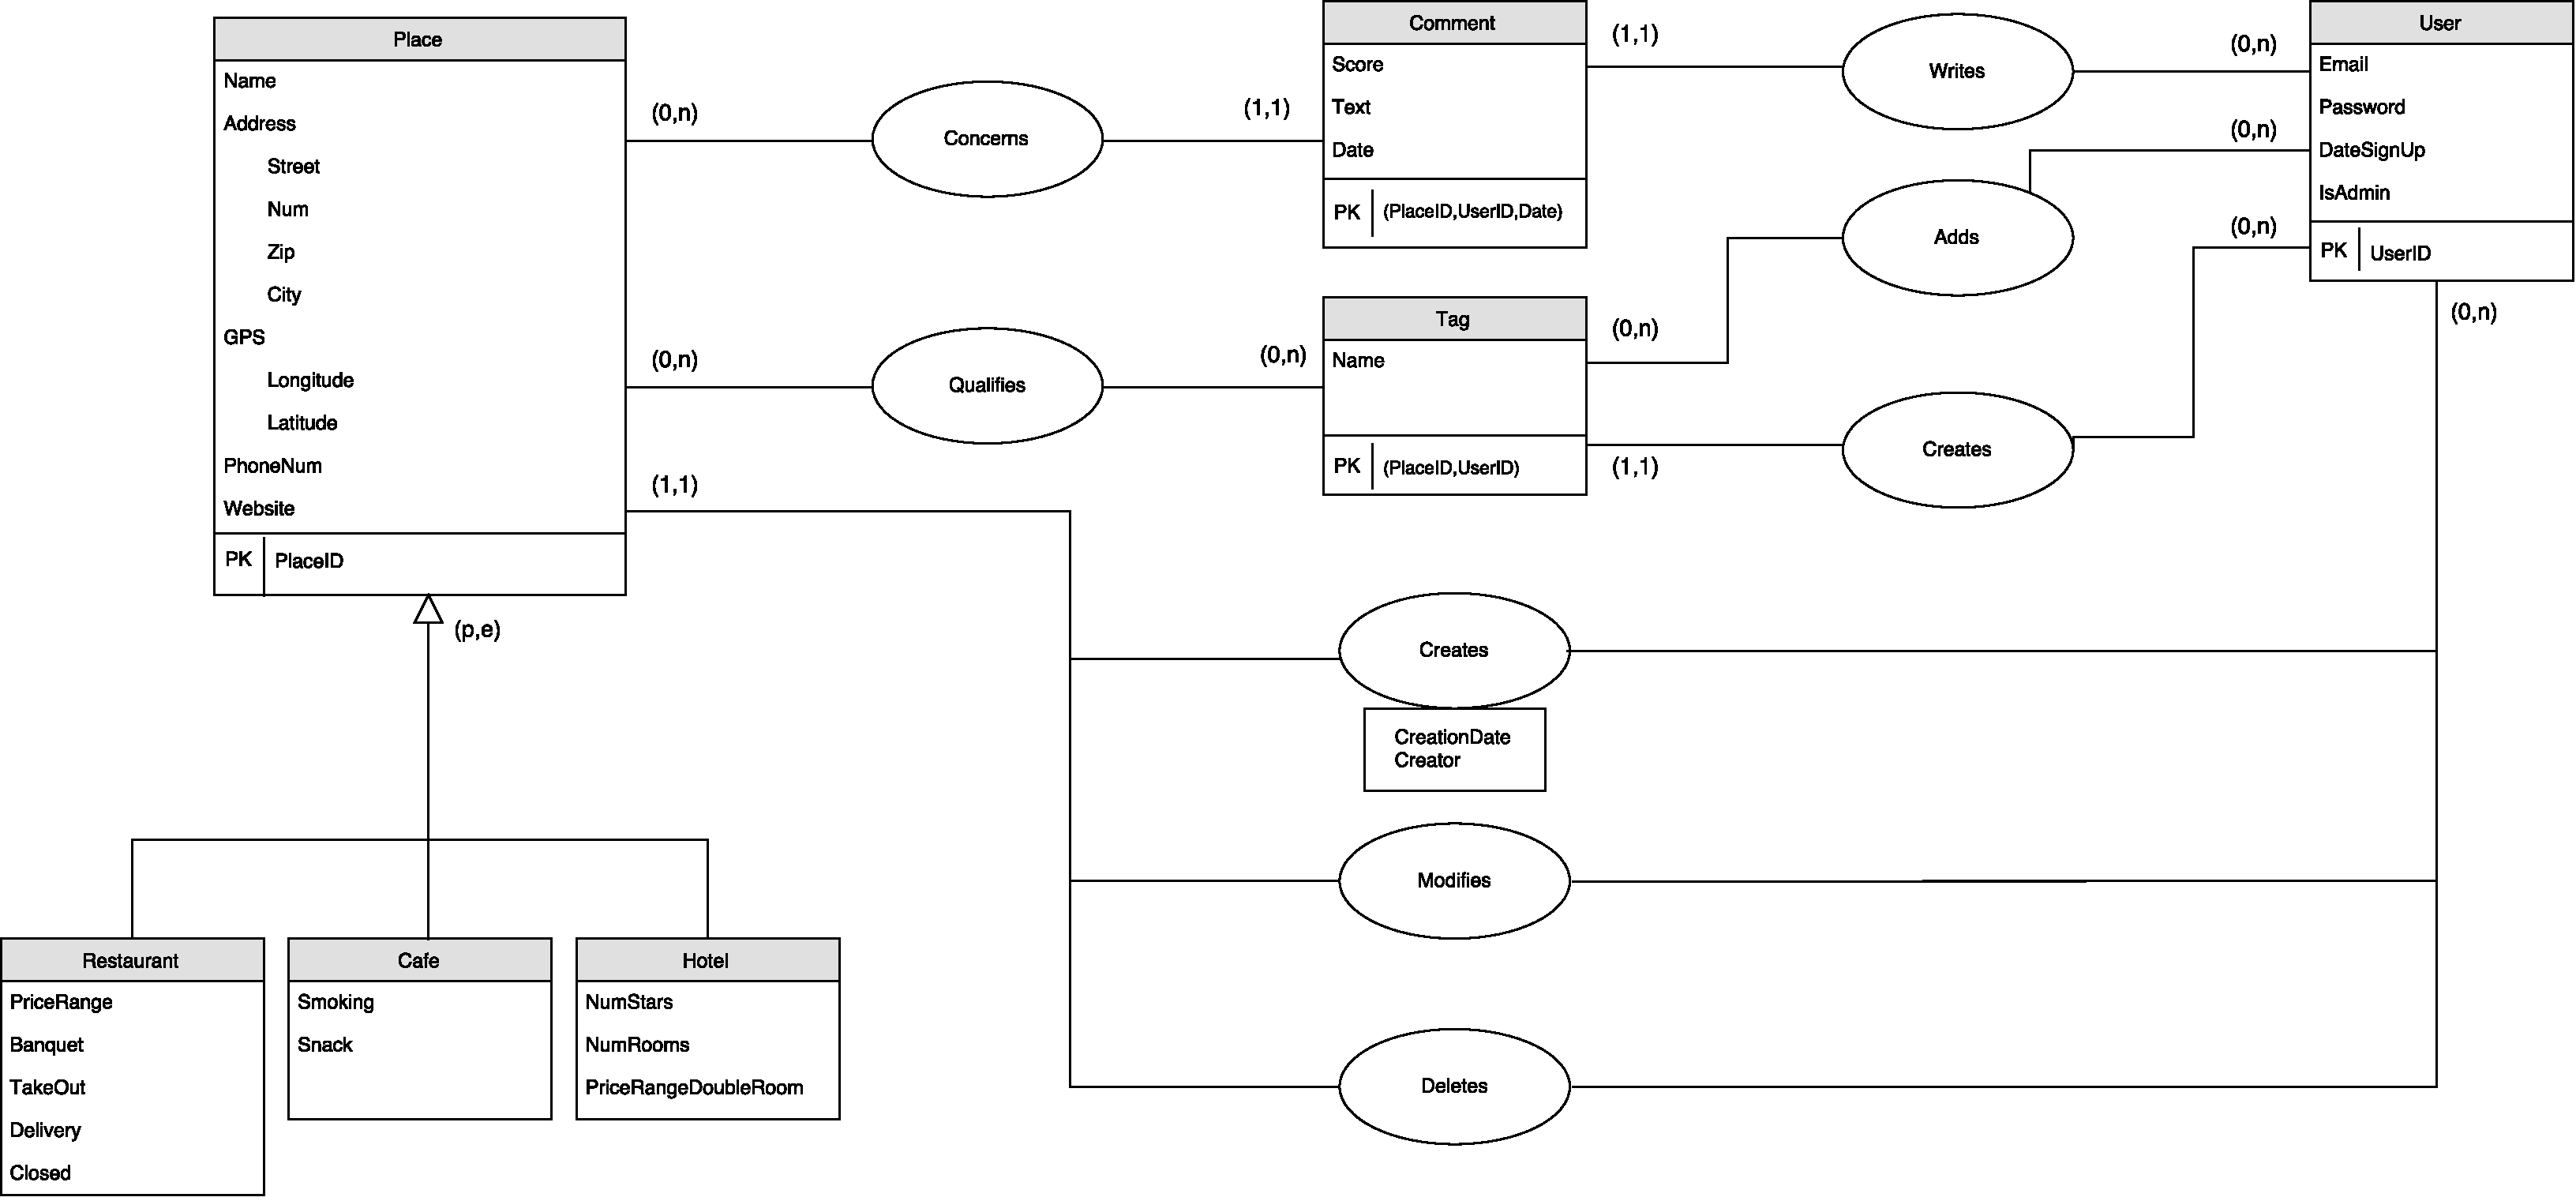
\includepdf[pages={-},angle=90,scale=0.75,pagecommand=\section{Diagramme entité-asssociation}]{./../erdiagrams/ERDia.pdf}

\section{Traduction relationnelle}

\noindent User(\underline{ID}, Email, Password, DateSignUp, IsAdmin)

\hspace{-0,5cm}Place(\underline{ID}, Name, Address, GPS, PhoneNum, Website)

\hspace{-0,5cm}Restaurant(\underline{PID}, PriceRange, Banquet, TakeOut, Delivery, Closed)

PID reference Place.ID

\hspace{-0,5cm}Cafe(\underline{PID}, Smoking, Snack)

PID reference Place.ID

\hspace{-0,5cm}Hotel(\underline{PID}, NumStars, NumRooms, PriceRangeDoubleRoom)

PID reference Place.ID

\hspace{-0,5cm}Comment(\underline{PID}, \underline{UID}, \underline{Date}, Score, Text, Date)

PID reference Place.ID

UID reference User.ID

\hspace{-0,5cm}Tag(\underline{PID}, \underline{UID}, Name)

PID reference Place.ID

UID reference User.ID

\hspace{-0,5cm}Creates(\underline{PID}, \underline{UID}, CreationDate)

PID reference Place.ID

UID reference User.ID



\section{Contraintes d'intégrité}

\begin{itemize}
  \item Pour pouvoir créer, modifier ou supprimer un "Place", le "User" doit être un administrateur (\emph{IsAdmin} == True).
  \item La \emph{Date} d'un "Comment" doit être strictement supérieure à la \emph{CreationDate} d'un "Place".
  \item La \emph{Date} d'un "Comment" doit être strictement supérieure à la \emph{DateSignUp} du "User" qui le poste.
  \item Il ne peut exister deux "Comment" d'un même "User" pour un même "Place" à la même \emph{Date}.
  \item La \emph{Note} d'un "Comment" doit être comprise entre 0 et 5 inclus.
  \item Les \emph{Name} des "Tag" doivent être uniques.
  \item Un "User" ne peut apposer plus d'une fois un "Tag" sur une même "Place".
  \item Tous les \emph{Email} des "User" doivent être uniques.
\end{itemize}

\end{document}
